\subsection{Effects on the $tV$ production}

Figure~\ref{fig:appB:pTV} and~\ref{fig:appB:pTtop} shows the $V$ mass distribution, the transverse momentum for $V$ and for the top quark coming from $V\to t\bar{u}$, for different masses and $V$ width. 
These figures are relevant independtly of the $V$ decay mode (visible or invisible). It applies then for both monotop and same-sign top final states.

\begin{figure}[!h!tpd]
  \centering
  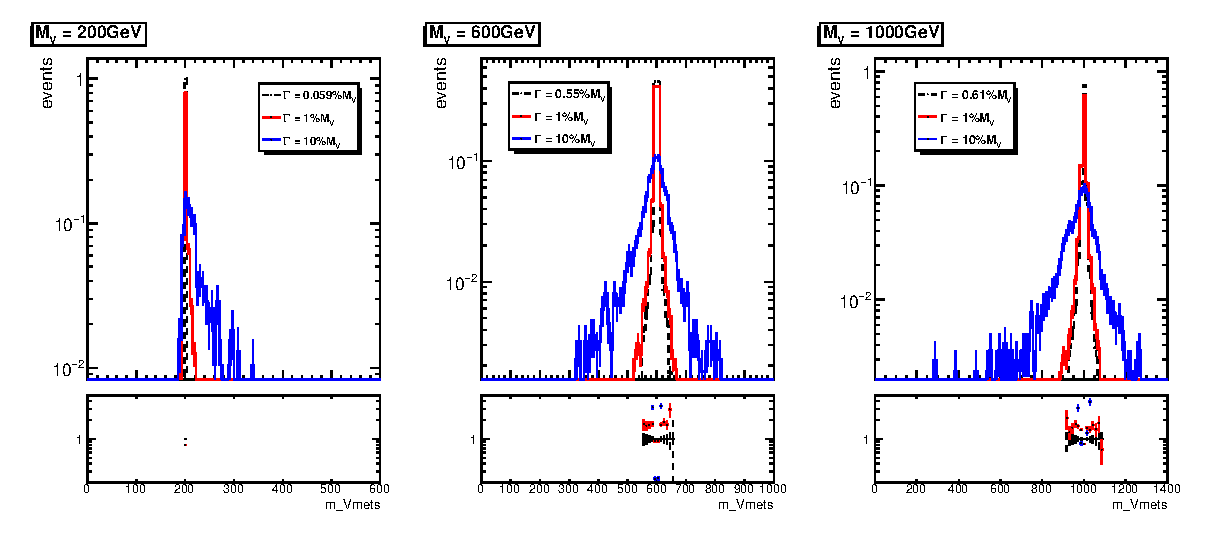
\includegraphics[width=1.0\textwidth]{appendix/appendixB/m_Vmets.eps}
  \caption{
    Distribution of $V$ invariant mass for the $gu\to tV(\to t\bar{u})$ (on-shell V) 
    for $m_V = \{200, 600, 1000\}~\GeV{}$ (from left to right) and for three different
    visible decay width (computed from Madgraph directly, $1\%$ and $10\%$).
  }   
  \label{fig:appB:Vmass}
\end{figure}


\begin{figure}[!h!tpd]
  \centering
  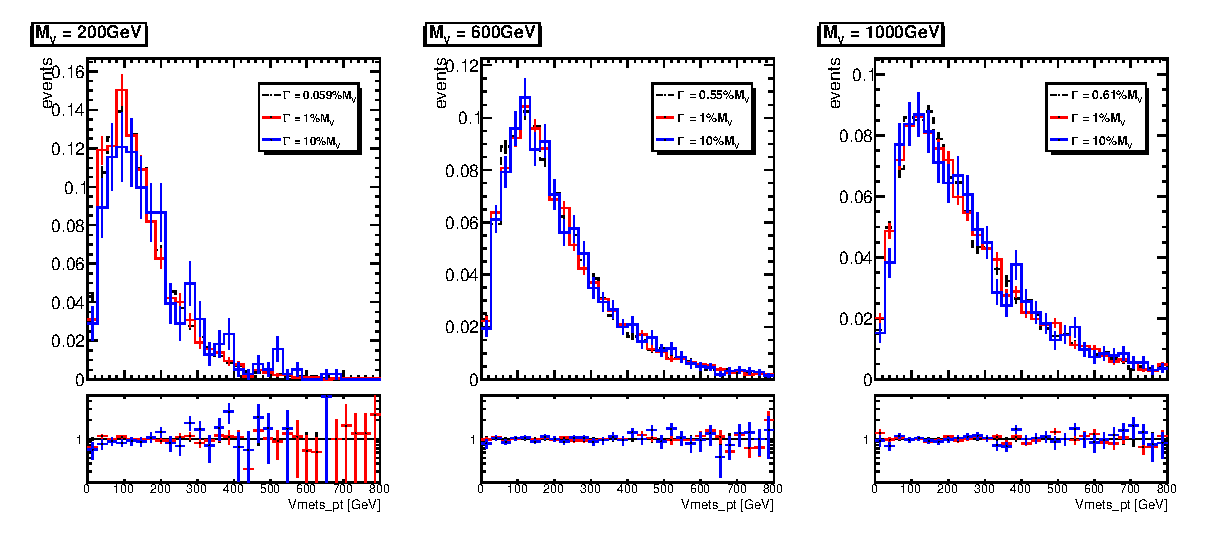
\includegraphics[width=1.0\textwidth]{appendix/appendixB/Vmets_pt.eps}
  \caption{
    Distribution of the $V$ $p_T$ for the $gu\to tV(\to t\bar{u})$ (on-shell V) for $m_V = \{200, 600, 1000\}~\GeV{}$ (from left to right) and for three different
    visible decay width (computed from Madgraph directly, $1\%$ and $10\%$).
  }
  \label{fig:appB:pTV}
\end{figure}


\begin{figure}[!h!tpd]
  \centering
  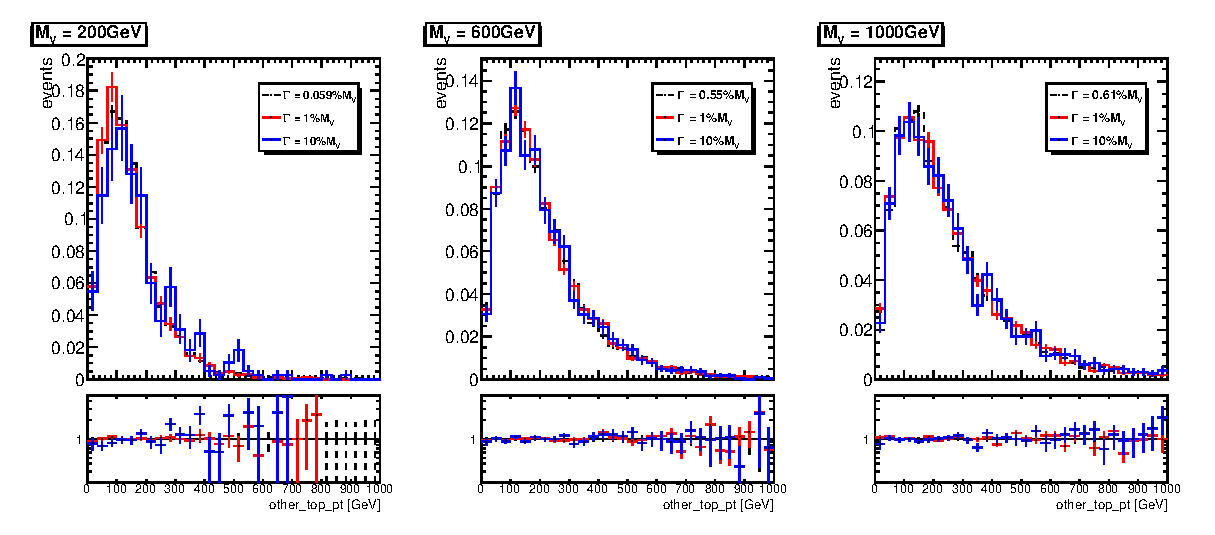
\includegraphics[width=1.0\textwidth]{appendix/appendixB/other_top_pt.eps}
  \caption{
    Distribution of the top quark $p_T$ produced in association with $V$ in $gu\to tV$ for $m_V = \{200, 600, 1000\}~\GeV{}$ (from left to right) and for three different
    visible decay width (computed from Madgraph directly, $1\%$ and $10\%$).
  }
  \label{fig:appB:pTtop}
\end{figure}



%\clearpage
\subsection{Effects on the $tt+X$ final state}
\label{sec:appB:ttXimpact}

Figures~\ref{fig:appB:pTAllTops} to~\ref{fig:appB:HT} focus on the $tt+X$ production showing the $p_T$ of all top quarks in the events, 
the leading jet $p_T$, the jet multiplicity, the $\met$, the lepton multiplicity and $H_T$. These plots
show that with $V$ width has a clear impact on some important distributions (top quark $p_T$, leading jet $p_T$, jet multiplicity, $H_T$). Section~\ref{sec:appB:tt_vs_tV} will 
demonstrate this impact is just a consequence of how the width change the relative fraction of each diagrams of Figure~\ref{fig:appA:feyn_prod_ss_all}.

\begin{figure}[!h!tpd]
  \centering
  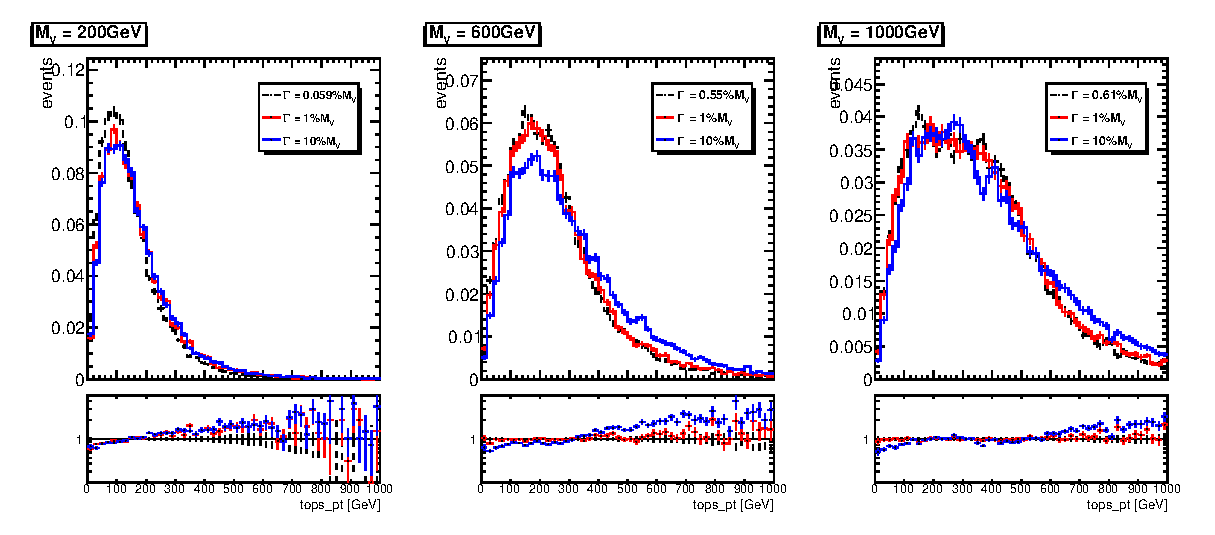
\includegraphics[width=1.0\textwidth]{appendix/appendixB/tops_pt.eps}
  \caption{
    Distribution of all top quark $p_T$ in the events for all processes leading to $tt+X$
    for $m_V = \{200, 600, 1000\}~\GeV{}$ (from left to right) and for three different
    visible decay width (computed from Madgraph directly, $1\%$ and $10\%$).
  }   
  \label{fig:appB:pTAllTops}
\end{figure}


\begin{figure}[!h!tpd]
  \centering
  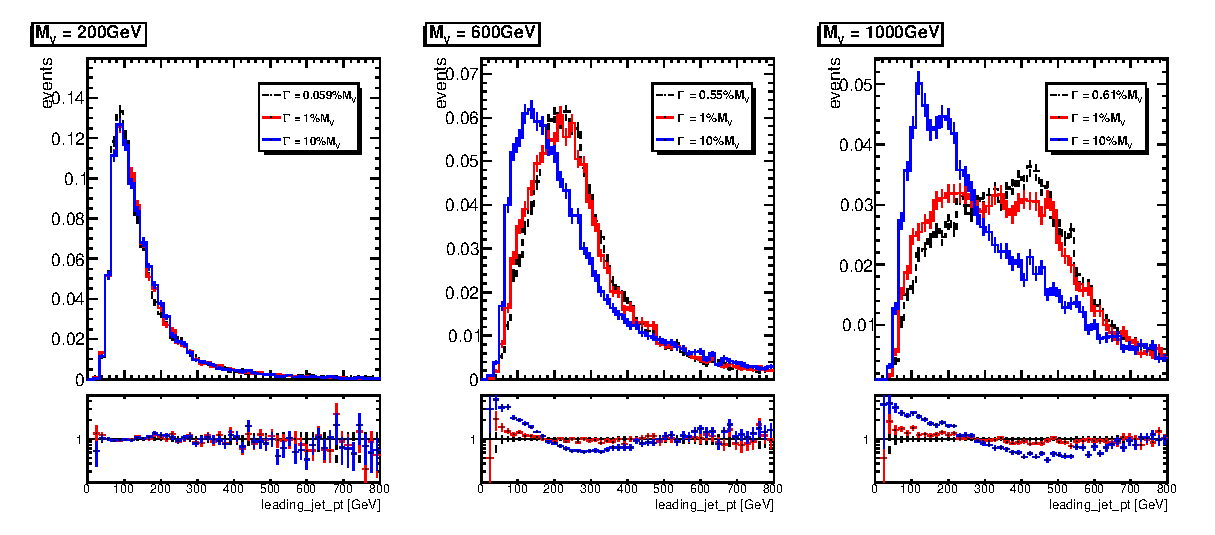
\includegraphics[width=1.0\textwidth]{appendix/appendixB/leading_jet_pt.eps}
  \caption{
      Distribution of the leading jet $p_T$ for all processes leading to $tt+X$
      for $m_V = \{200, 600, 1000\}~\GeV{}$ (from left to right) and for three different
      visible decay width (computed from Madgraph directly, $1\%$ and $10\%$).
  }   
  \label{fig:appB:Vmass}
\end{figure}


\begin{figure}[!h!tpd]
  \centering
  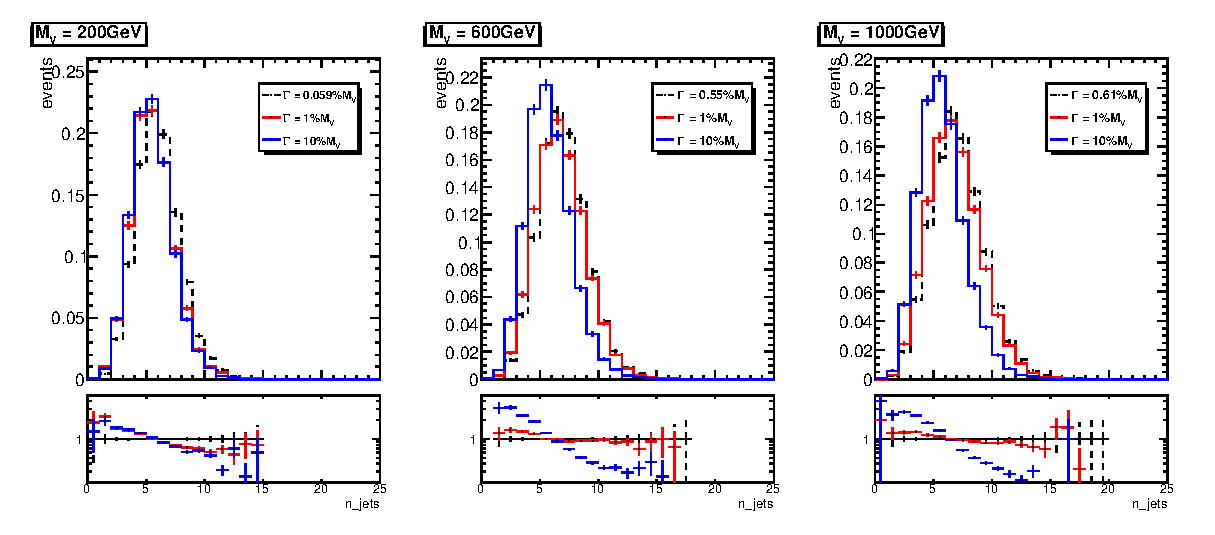
\includegraphics[width=1.0\textwidth]{appendix/appendixB/n_jets.eps}
  \caption{
      Distribution of the jet multiplicity for all processes leading to $tt+X$
      for $m_V = \{200, 600, 1000\}~\GeV{}$ (from left to right) and for three different
      visible decay width (computed from Madgraph directly, $1\%$ and $10\%$).
  }   
  \label{fig:appB:Vmass}
\end{figure}


\begin{figure}[!h!tpd]
  \centering
  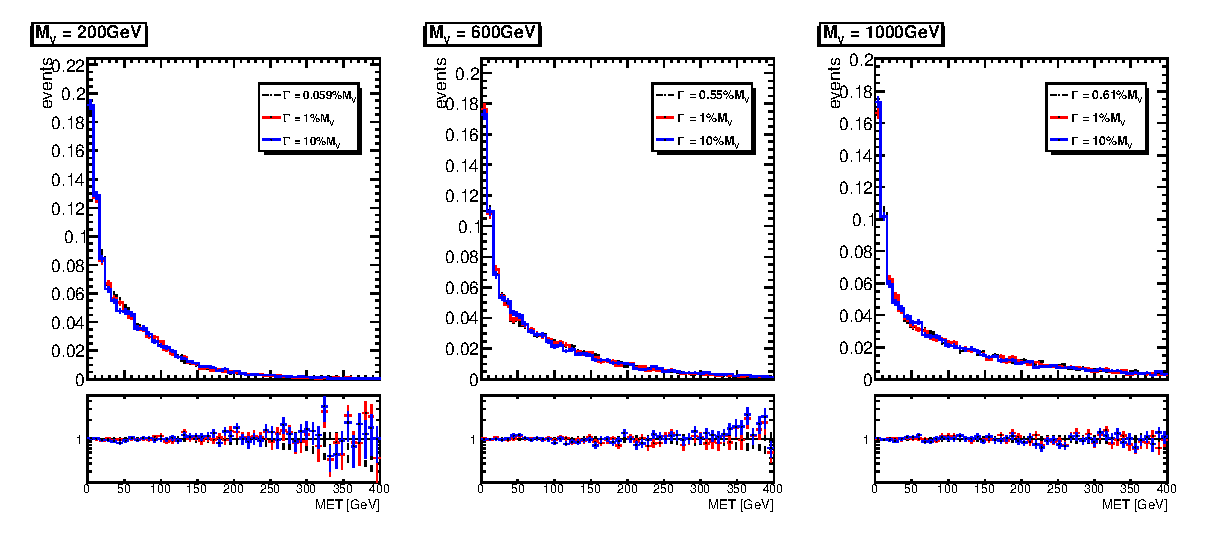
\includegraphics[width=1.0\textwidth]{appendix/appendixB/MET.eps}
  \caption{
      Distribution of the $\met$ for all processes leading to $tt+X$
      for $m_V = \{200, 600, 1000\}~\GeV{}$ (from left to right) and for three different
      visible decay width (computed from Madgraph directly, $1\%$ and $10\%$).
  }   
  \label{fig:appB:Vmass}
\end{figure}



\begin{figure}[!h!tpd]
  \centering
  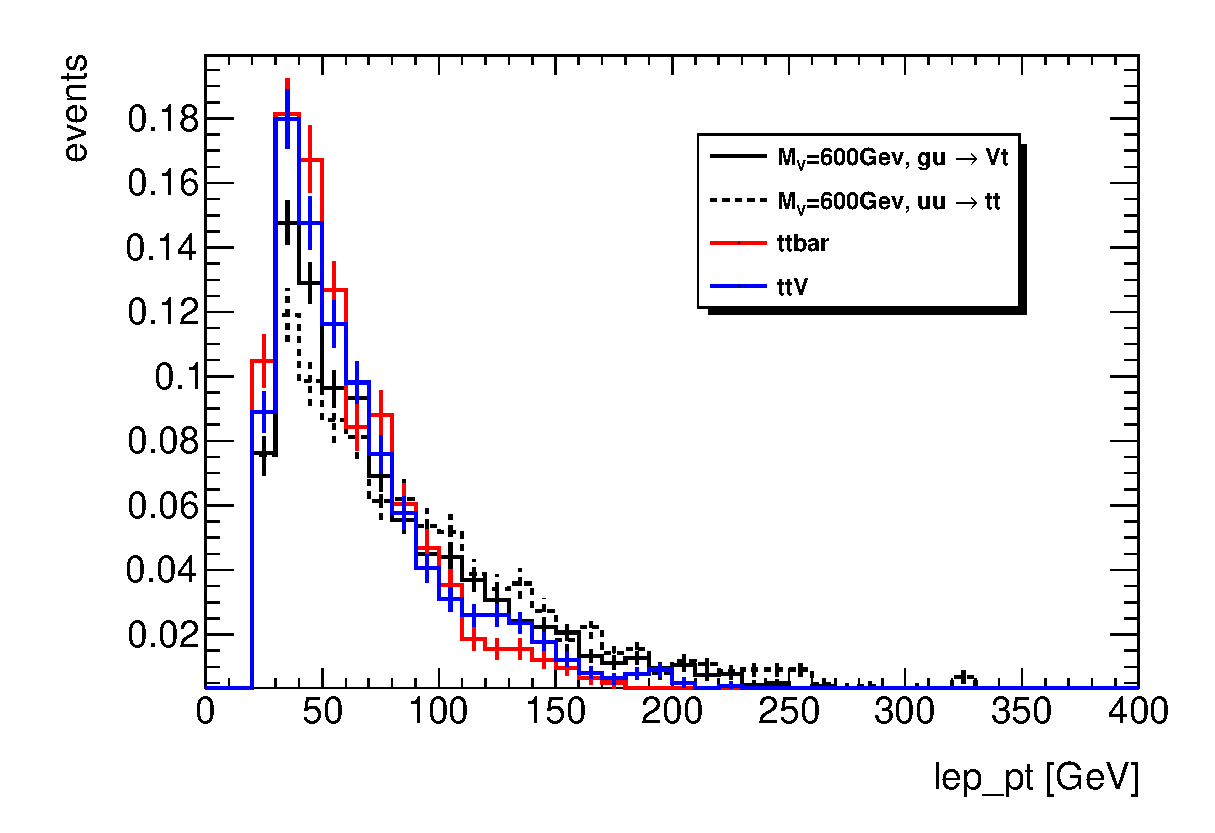
\includegraphics[width=1.0\textwidth]{appendix/appendixB/lep_pt.eps}
  \caption{
      Distribution of the lepton $p_T$ for all processes leading to $tt+X$
      for $m_V = \{200, 600, 1000\}~\GeV{}$ (from left to right) and for three different
      visible decay width (computed from Madgraph directly, $1\%$ and $10\%$).
  }   
  \label{fig:appB:Vmass}
\end{figure}


\begin{figure}[!h!tpd]
  \centering
  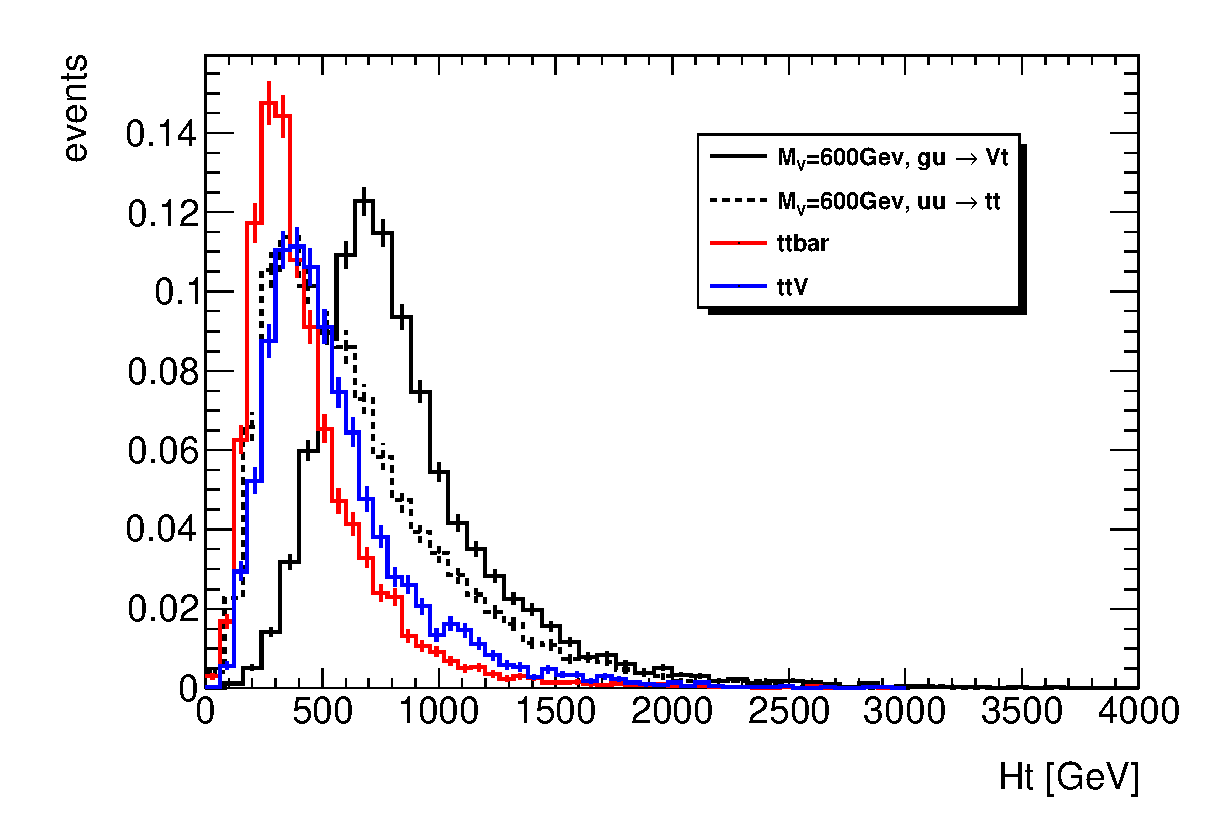
\includegraphics[width=1.0\textwidth]{appendix/appendixB/Ht.eps}
  \caption{
      Distribution of the $p_T$ scalar sum ($H_T$) for all processes leading to $tt+X$
      for $m_V = \{200, 600, 1000\}~\GeV{}$ (from left to right) and for three different
      visible decay width (computed from Madgraph directly, $1\%$ and $10\%$).
  }   
  \label{fig:appB:HT}
\end{figure}


\clearpage
\subsection{Comparison of $gu \to tV(\to t\bar{u})$ and $uu\to tt$ processes}
\label{sec:appB:tt_vs_tV}

Figures~\ref{fig:appB:pTAllTops_stchannel} to~\ref{fig:appB:HT_stchannel} show the width effect on top $p_T$, leading jet $p_T$, jet multiplicity and $H_T$, 
separately for $gu \to tV(\to t\bar{u})$ and $uu \to tt$ processes. These plot show the important kinematic differences between the $tt$ production 
via a $t$-channel exchange of the mediator and the direct production of the mediator, decaying into $t\bar{u}$. On each of these process, the width doesn't
change at all the kinematics but it does change the relative importance of each process, as shown in section~\ref{sec:appA}. This explains then the
width impact observed in section~\ref{sec:appB:ttXimpact}.


\begin{figure}[!h!tpd]
  \centering
  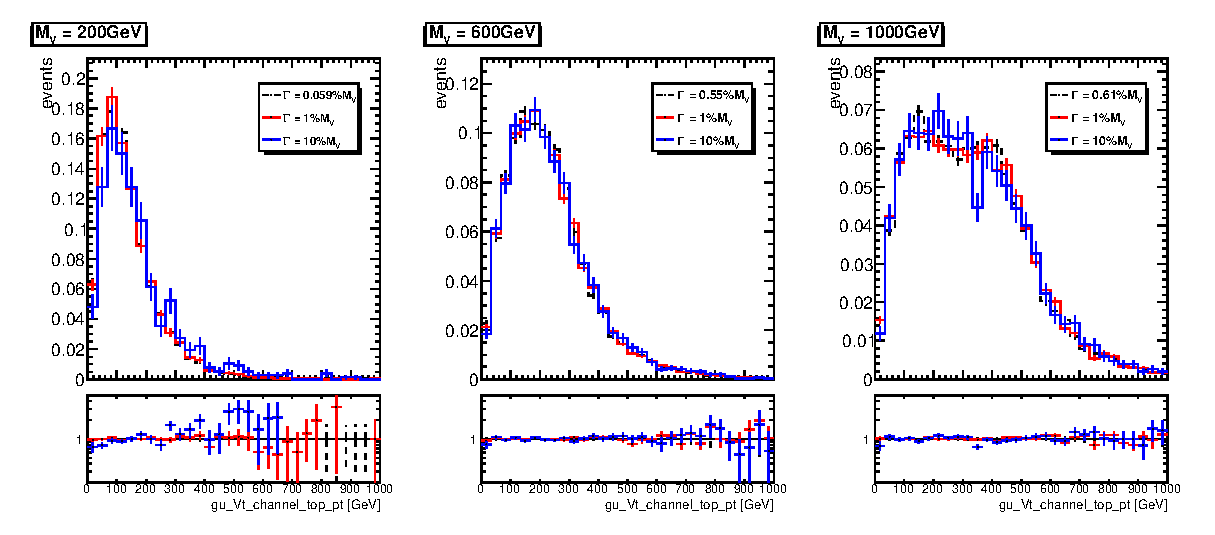
\includegraphics[width=1.0\textwidth]{appendix/appendixB/gu_Vt_channel_top_pt.eps} \\
  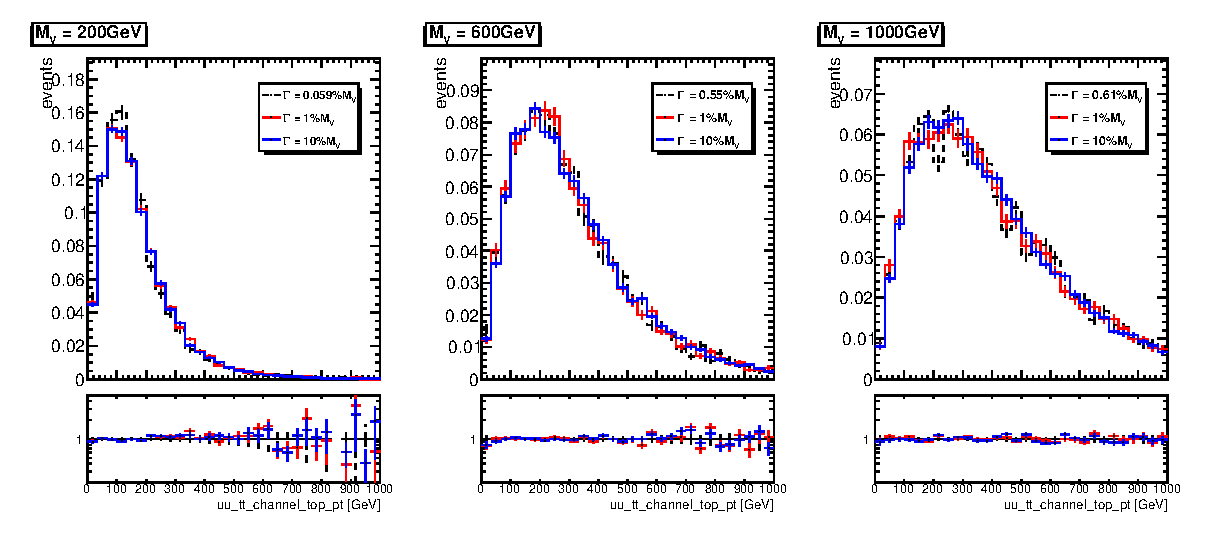
\includegraphics[width=1.0\textwidth]{appendix/appendixB/uu_tt_channel_top_pt.eps}
  \caption{
      Distribution of all top quark $p_T$ in the events for all processes leading to $tt+X$
      for $m_V = \{200, 600, 1000\}~\GeV{}$ (from left to right) and for three different
      visible decay width (computed from Madgraph directly, $1\%$ and $10\%$). Top plots show $gu \to tt \bar{u}$ and bottom plots show $uu \to tt$.
  }   
  \label{fig:appB:pTAllTops_stchannel}
\end{figure}


\begin{figure}[!h!tpd]
  \centering
  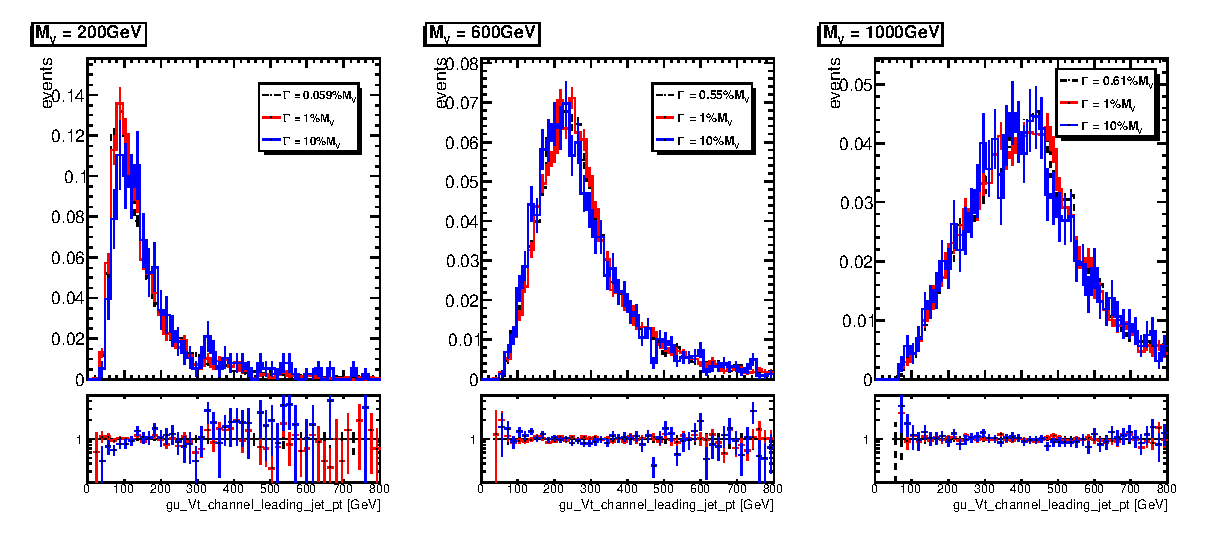
\includegraphics[width=1.0\textwidth]{appendix/appendixB/gu_Vt_channel_leading_jet_pt.eps}\\
  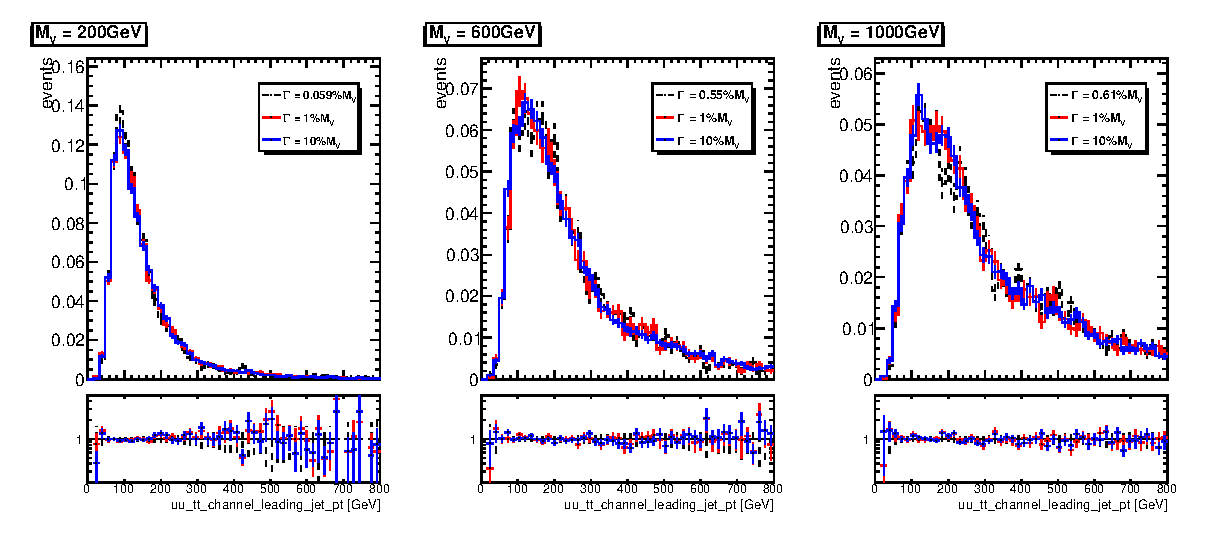
\includegraphics[width=1.0\textwidth]{appendix/appendixB/uu_tt_channel_leading_jet_pt.eps}
  \caption{
      Distribution of the leading jet $p_T$ for all processes leading to $tt+X$
      for $m_V = \{200, 600, 1000\}~\GeV{}$ (from left to right) and for three different
      visible decay width (computed from Madgraph directly, $1\%$ and $10\%$). Top plots show $gu \to tt \bar{u}$ and bottom plots show $uu \to tt$.
  }   
  \label{fig:appB:Vmass}
\end{figure}


\begin{figure}[!h!tpd]
  \centering
  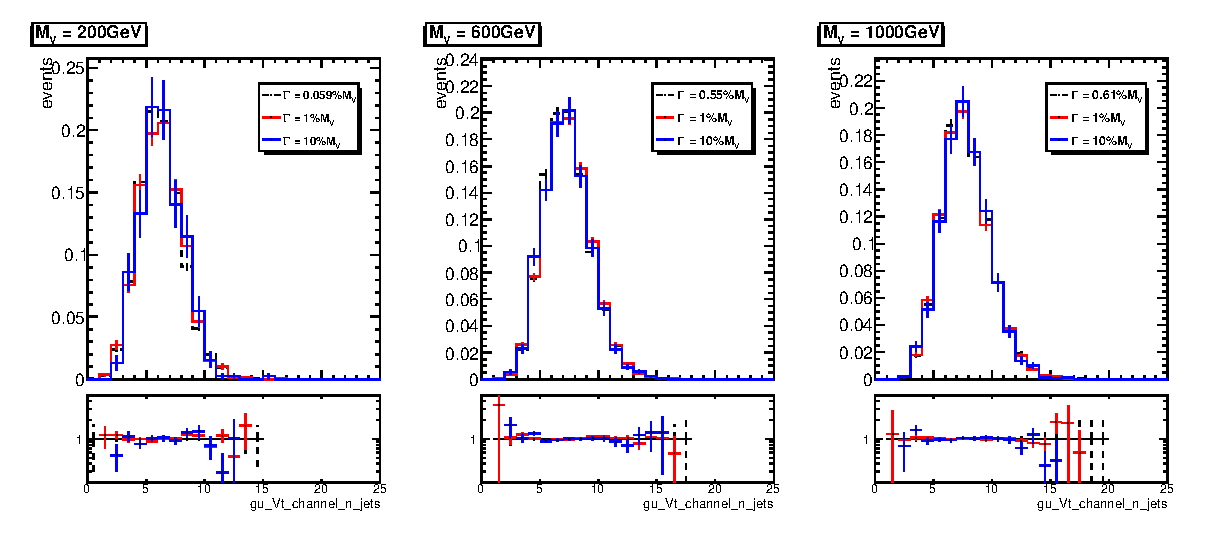
\includegraphics[width=1.0\textwidth]{appendix/appendixB/gu_Vt_channel_n_jets.eps}\\
  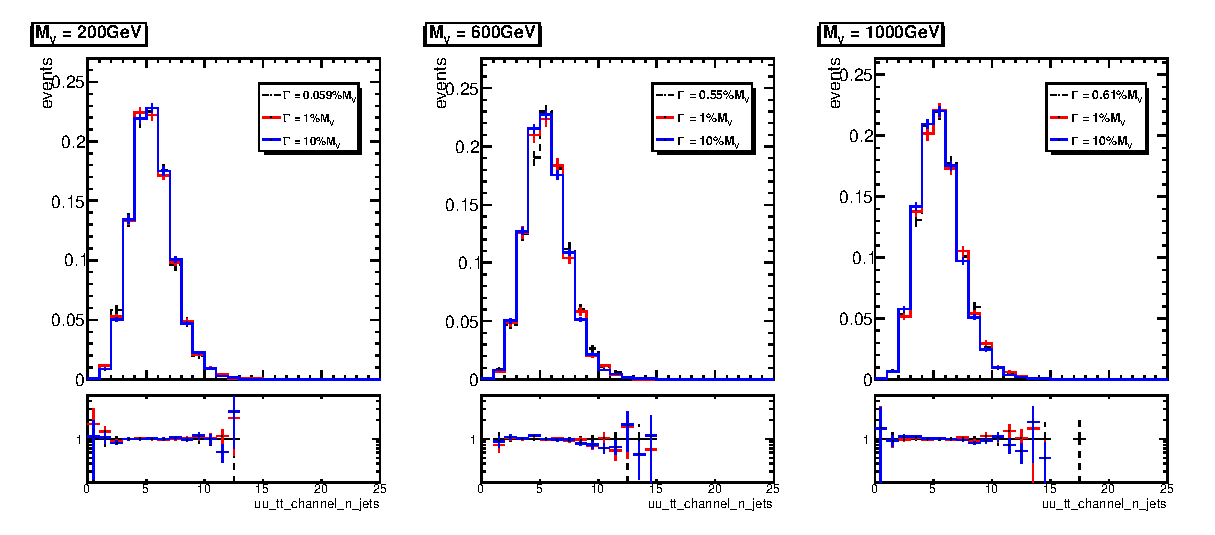
\includegraphics[width=1.0\textwidth]{appendix/appendixB/uu_tt_channel_n_jets.eps}
  \caption{
      Distribution of the jet multiplicity for all processes leading to $tt+X$
      for $m_V = \{200, 600, 1000\}~\GeV{}$ (from left to right) and for three different
      visible decay width (computed from Madgraph directly, $1\%$ and $10\%$). Top plots show $gu \to tt \bar{u}$ and bottom plots show $uu \to tt$.
  }   
  \label{fig:appB:Vmass}
\end{figure}

\begin{figure}[!h!tpd]
  \centering
  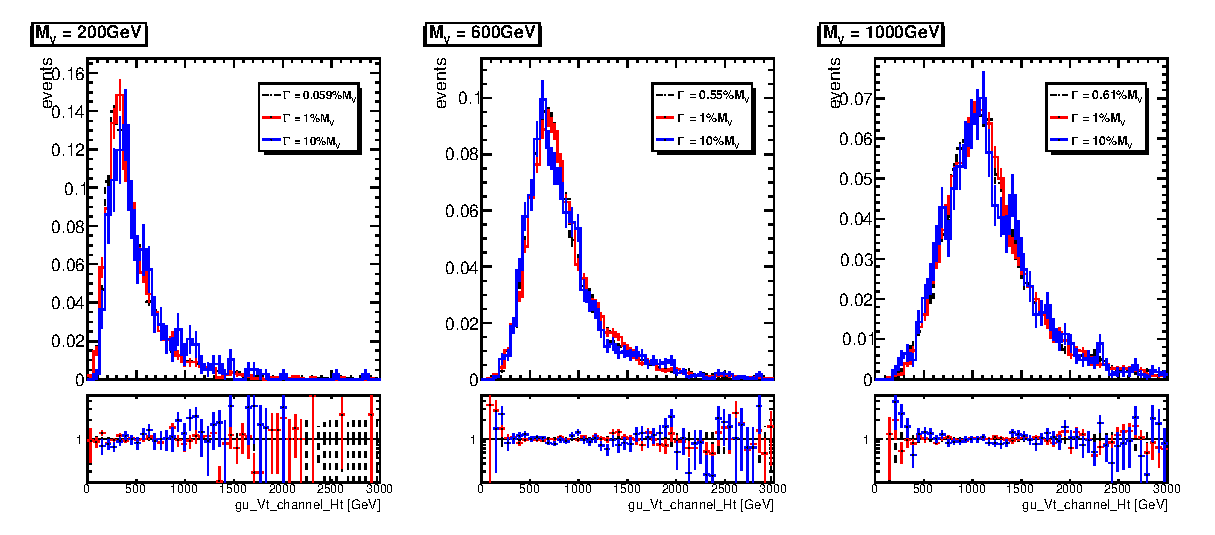
\includegraphics[width=1.0\textwidth]{appendix/appendixB/gu_Vt_channel_Ht.eps}\\
  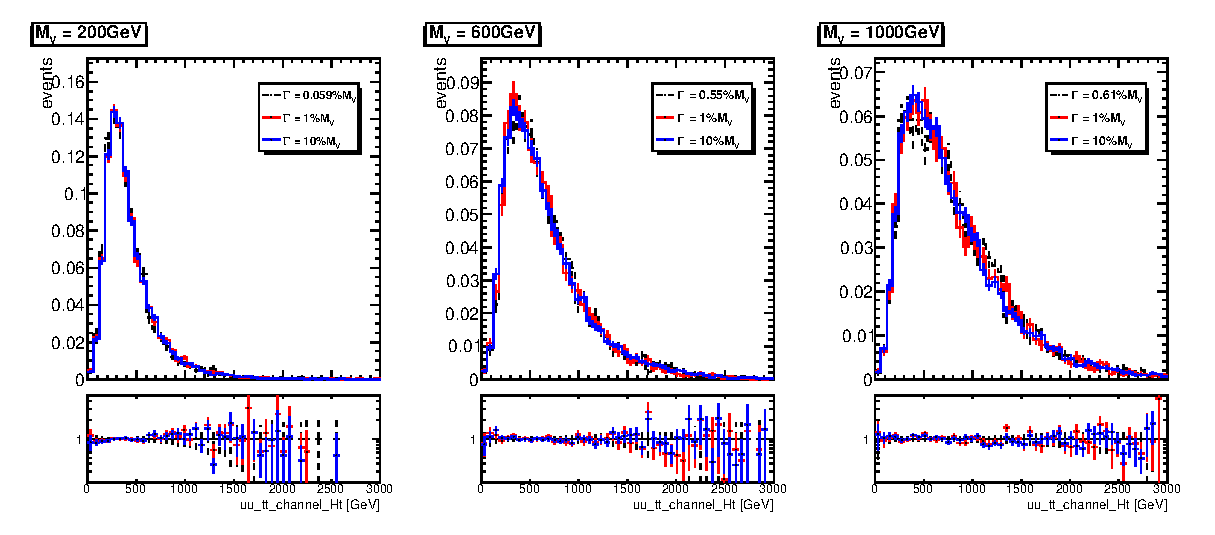
\includegraphics[width=1.0\textwidth]{appendix/appendixB/uu_tt_channel_Ht.eps}
  \caption{
    Distribution of the $p_T$ scalar sum ($H_T$) for all processes leading to $tt+X$
    for $m_V = \{200, 600, 1000\}~\GeV{}$ (from left to right) and for three different
    visible decay width (computed from Madgraph directly, $1\%$ and $10\%$). Top plots show $gu \to tt \bar{u}$ and bottom plots show $uu \to tt$.
  }   
  \label{fig:appB:HT_stchannel}
\end{figure}

